\section*{Resultater}
\label{Resultater}
%
Ud fra det udarbejdede \textit{affinity diagram} udvælges de to grønne, overordnede kategorier, der er relevante i forhold til dette mini projekt, som er: \textit{Robottens udseende}, illustreret på \autoref{fig:RsUdseende}, samt \textit{Robottens væremåde}, illustreret på \autoref{fig:RsVaeremaade}.
%
\begin{figure}[H]
\centering
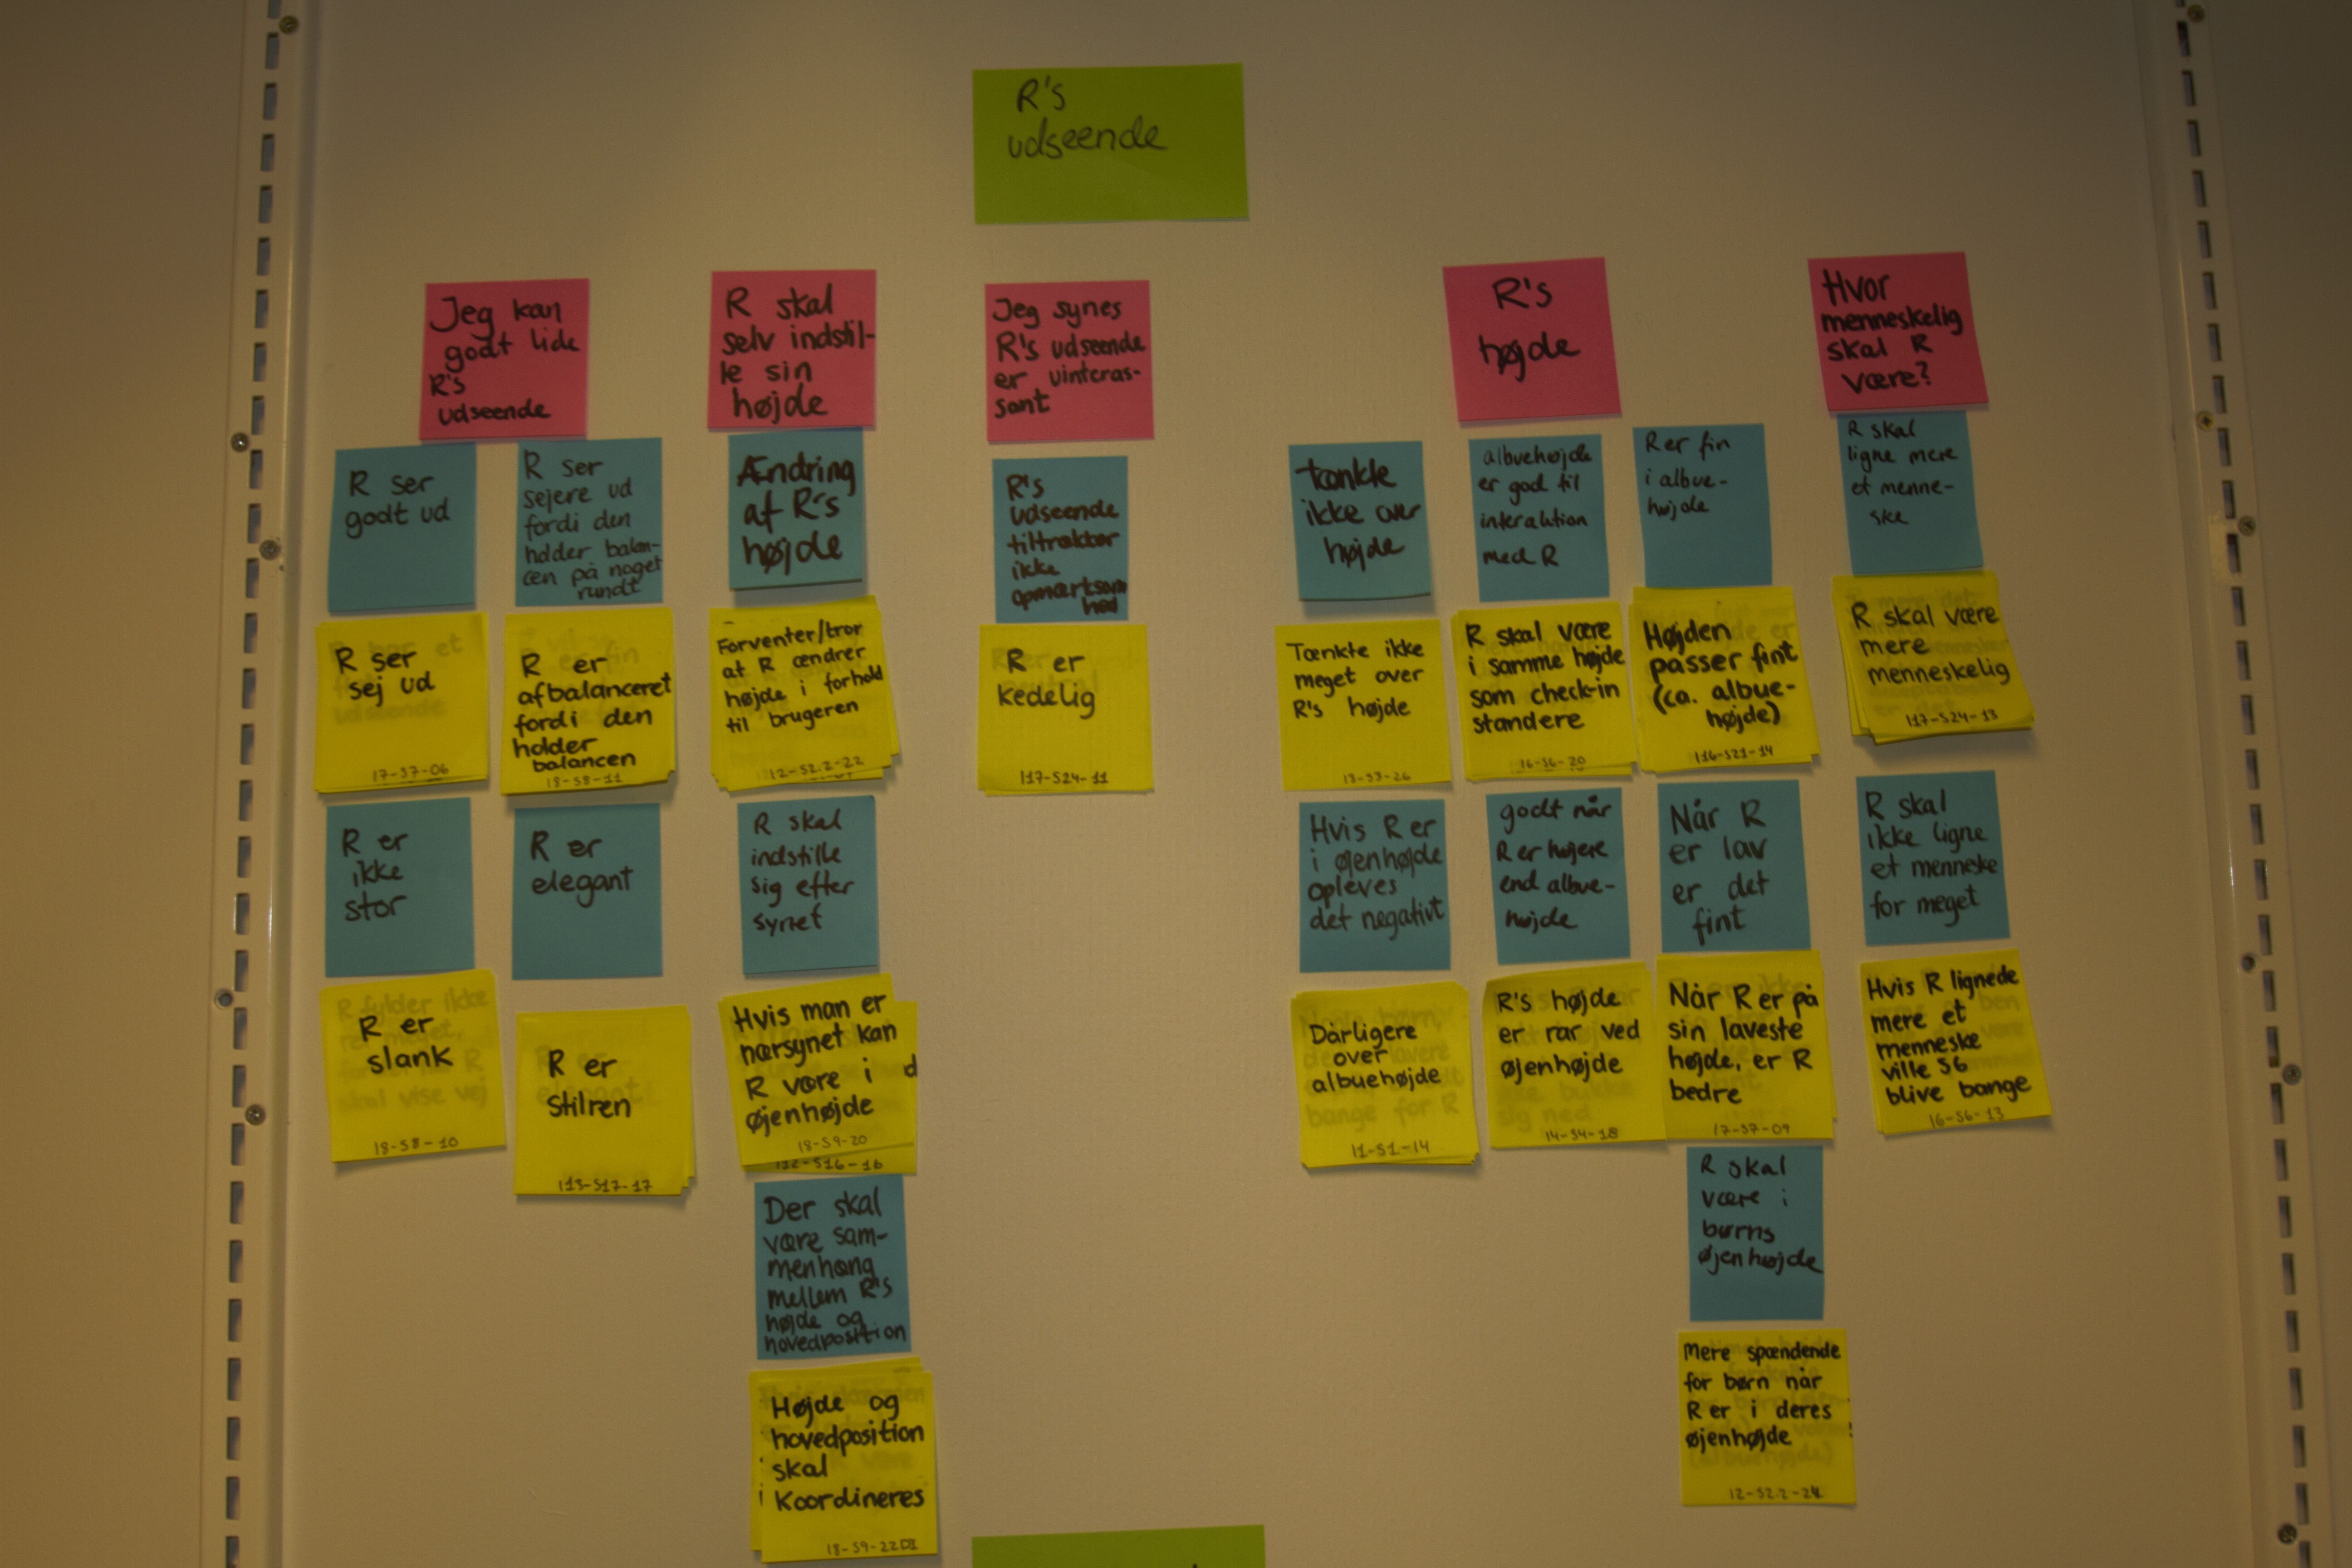
\includegraphics[width = 0.9\textwidth]{Figure/RsUdseende} 
\caption{Udsnit af det samlede \textit{affinity diagram}, som vedrører robottens udseende.}
\label{fig:RsUdseende}
\end{figure}
\noindent
%
Da dette miniprojekt bygger på data indsamlet i forbindelse med semesterprojektet, er det ikke alle kategorier, der er angivet med pink labels, som har relevans for miniprojektet. I henhold til miniprojektet er det kun to af de pink labels, som kan anses for at være objektive attributter: \textit{R's højde} samt \textit{Hvor menneskelig skal R være?}, hvor R er en forkortelse for robot. I begge tilfælde er det muligt at ændre robottens fysiske karakteristika i forhold til højde og hvor menneskelig robotten perciperes. 
%
\begin{figure}[H]
\centering
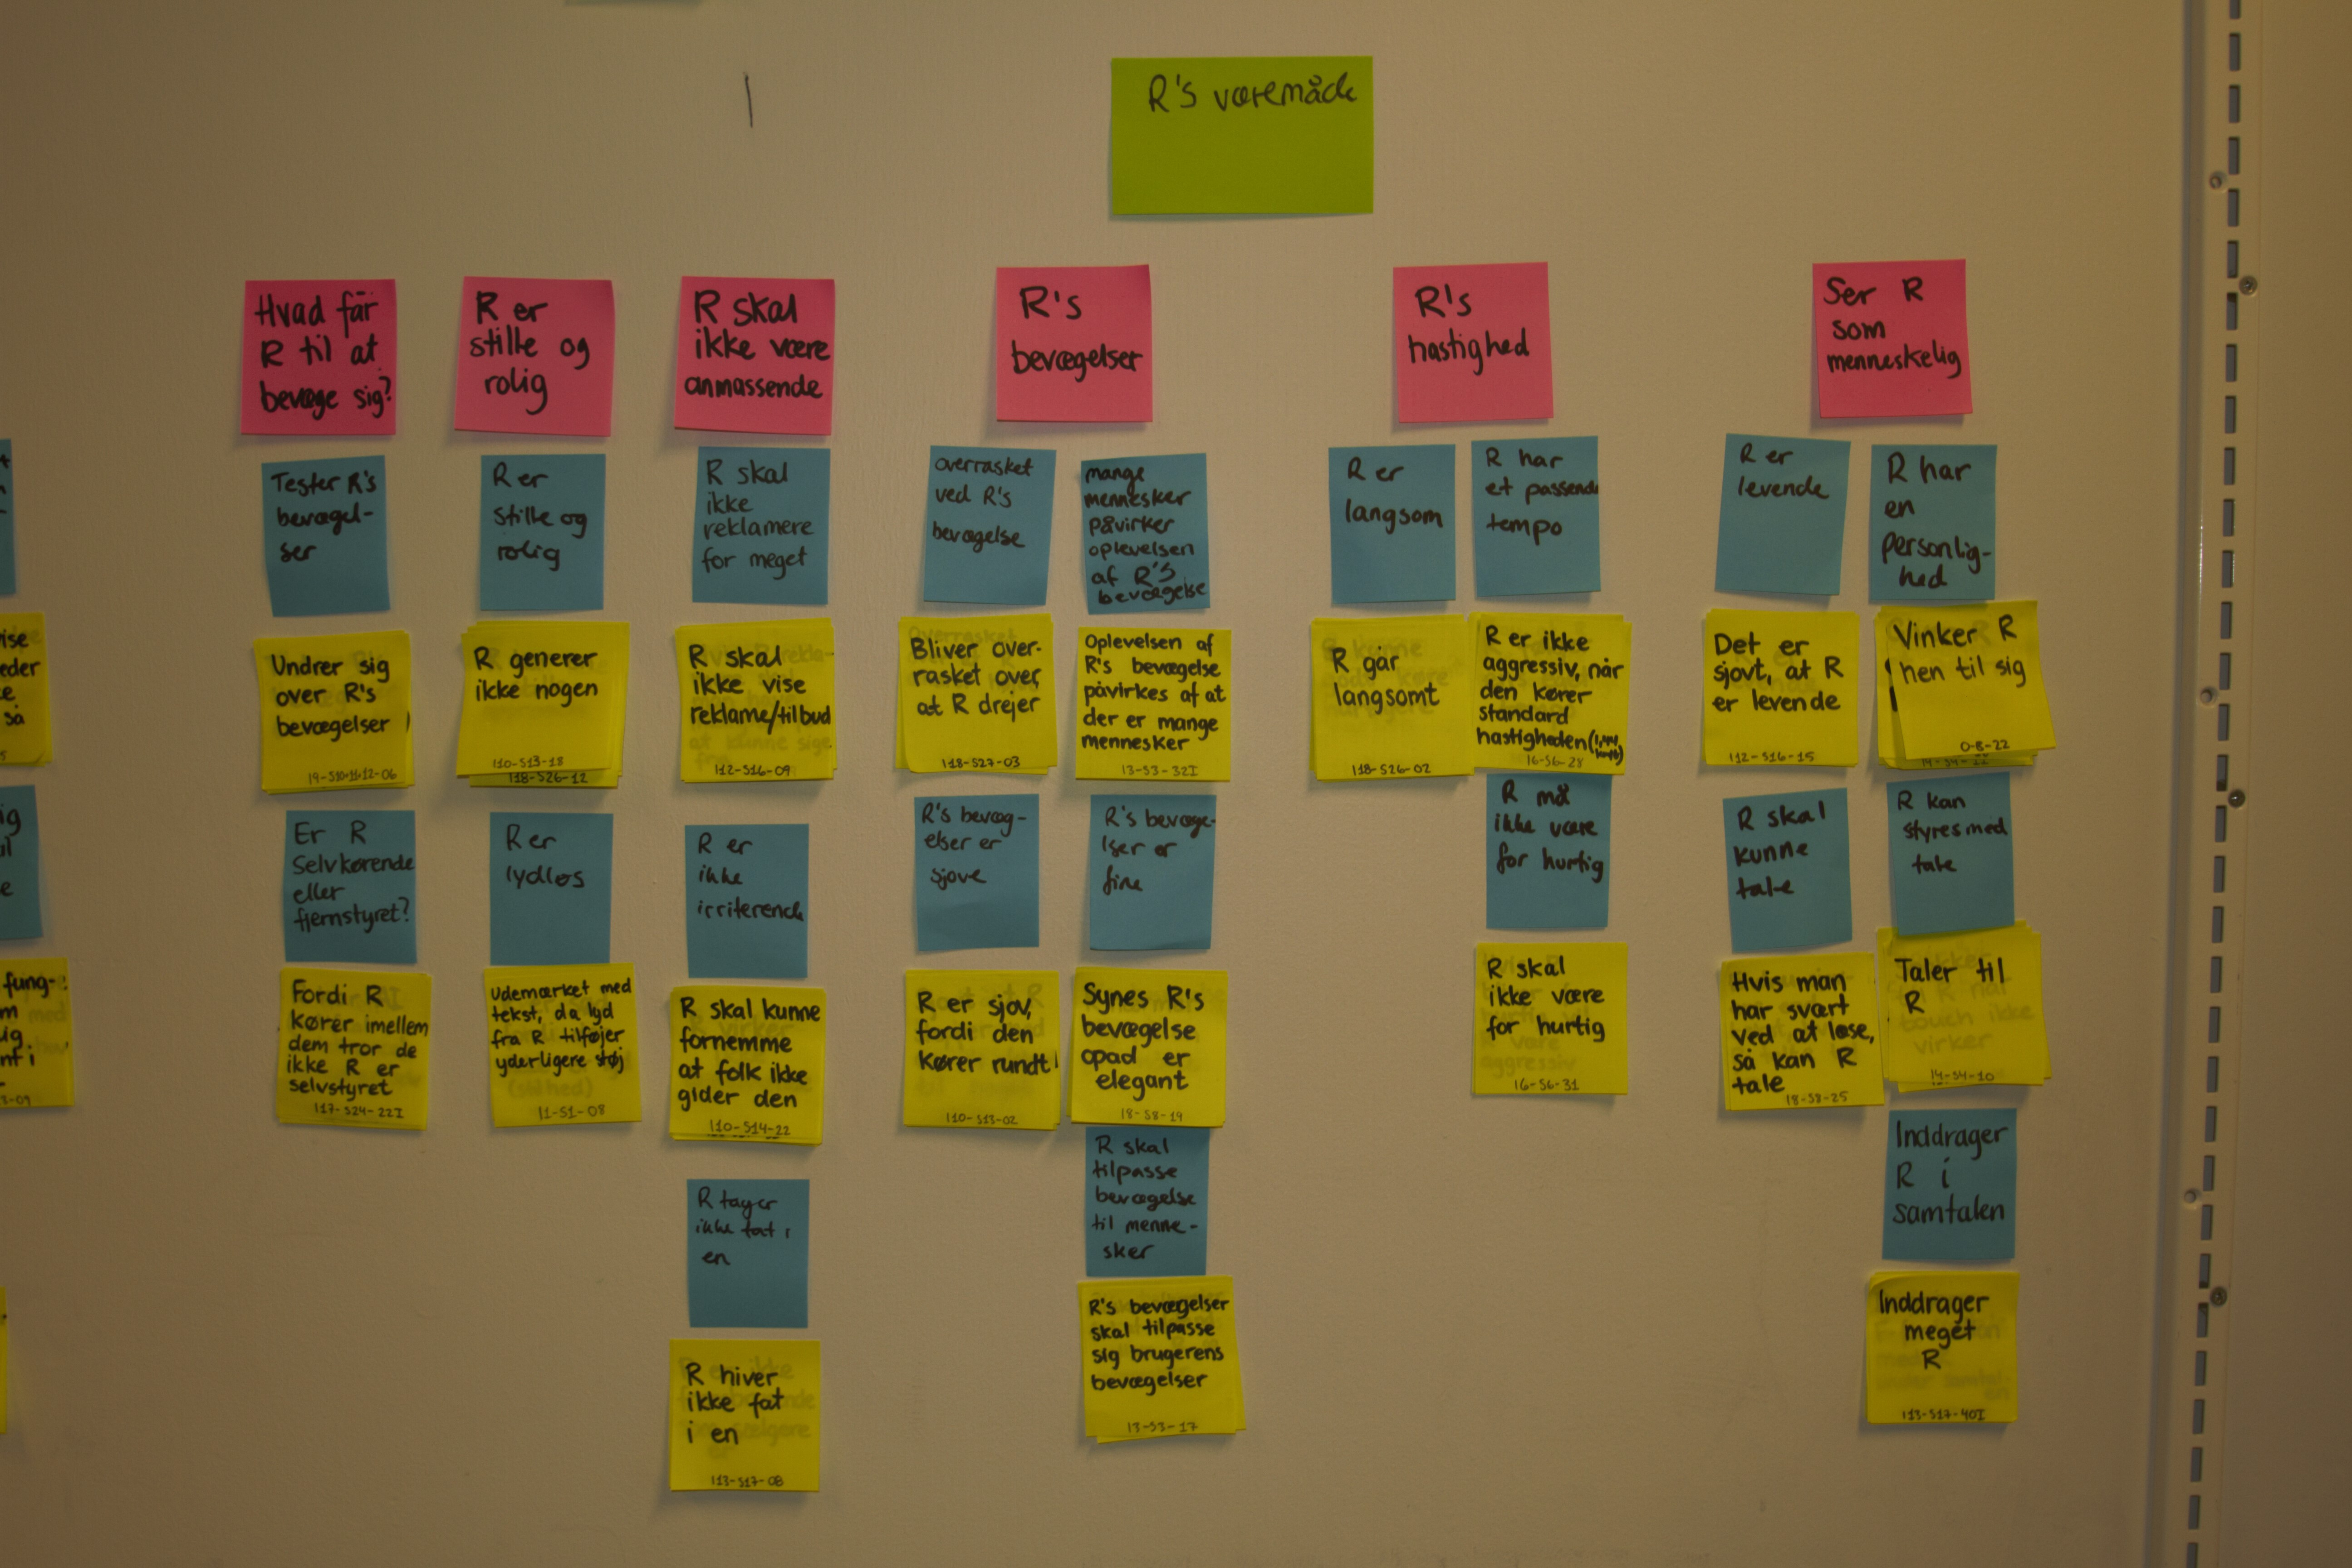
\includegraphics[width = 0.9\textwidth]{Figure/RsVaeremaade} 
\caption{Udsnit af det samlede \textit{affinity diagram}, som vedrører robottens væremåde.}
\label{fig:RsVaeremaade}
\end{figure}
\noindent
%
Ud af de seks pink kategorier, der fremgår på \autoref{fig:RsVaeremaade}, vil følgende kategorier inkluderes i miniprojektsammenhæng: \textit{R's bevægelser}, \textit{R's hastighed} samt \textit{Ser R som menneskelig}. Sidstnævnte kategori vedrører den samme attribut, som blev valgt fra \autoref{fig:RsUdseende}, hvorfor de to vil betragtes som værende én attribut som kan evalueres på flere skalaer. Selvom den pink label: \textit{R skal ikke være anmassende} er præferencebetonet vil det stadig blive inddraget i miniprojektet, da det er muligt at udvikle en skala som evaluerer en objektiv attribut, som henvender sig til hvorvidt robotten er anmassende.  

\subsection*{Udvikling af skala}
\label{UdviklingSkala}
%
Fælles for de efterfølgende skalaer er at de alle er udviklet som \textit{Visual Analoge Scale}, VAS, med åbne endepunkter. Er skalaen bipolær vil der være markeret et midterpunkt med en vertikal linje, hvorhvis skalaen er unipolær vil der ikke markeres et midterpunkt. 

Baseret på kategorierne: \textit{R's væremåde} og \textit{R's udseende}, kan følgende objektive attributter udledes til hver af de tre karakteristikas: \blankline
%
\begin{itemize}
  \item Bevægelse
  \item Henvendelse
  \item Udseende\blankline
\end{itemize}
%
I henhold til at evaluere robottens bevægelser, vil der være flere attributter i spil, hvor skalaerne afbilledes på \autoref{fig:KluntetElegant}, \autoref{fig:AggressivFredsommelig}, \autoref{fig:MenneskeligBevaegelse} og \autoref{fig:Hastighed}.
%
\begin{figure}[H]
\centering

\includegraphics[width =\textwidth]{Figure/KluntetElegant} 
\caption{Bipolær skala til at evaluere om robotten bevæger sig kluntet eller elegant.}
\label{fig:KluntetElegant}
\end{figure}
\noindent
%
%
\begin{figure}[H]
\centering

\includegraphics[width =\textwidth]{Figure/AggressivFredsommelig} 
\caption{Bipolær skala til at evaluere om robotten bevæger sig aggressivt.}
\label{fig:AggressivFredsommelig}
\end{figure}
\noindent
%
%
\begin{figure}[H]
\centering

\includegraphics[width =\textwidth]{Figure/Menneskelig} 
\caption{Unipolær skala til at evaluere om robotten bevæger sig menneskeligt.}
\label{fig:MenneskeligBevaegelse}
\end{figure}
\noindent
%
%
\begin{figure}[H]
\centering

\includegraphics[width =\textwidth]{Figure/Hastighed} 
\caption{Bipolær skala til at evaluere robottens hastighed.}
\label{fig:Hastighed}
\end{figure}
\noindent
%
I henhold til at evaluere robottens henvendelse vil der være flere attributter i spil, hvor skalaerne afbilledes på \autoref{fig:AnmassendeTilbageholden} og \autoref{fig:Henvendelse}.  
%
\begin{figure}[H]
\centering

\includegraphics[width =\textwidth]{Figure/AnmasendeTilbageholden} 
\caption{Bipolær skala til at evaluere om robotten bevæger sig aggressivt eller tilbageholdende.}
\label{fig:AnmassendeTilbageholden}
\end{figure}
\noindent
%
%
\begin{figure}[H]
\centering

\includegraphics[width =\textwidth]{Figure/Henvendelse} 
\caption{Bipolær skala til at evaluere robottens afstand til testpersonen.}
\label{fig:Henvendelse}
\end{figure}
\noindent
%
I henhold til at evaluere robottens udseende vil der være flere attributter i spil, hvor skalaerne afbilledes på \autoref{fig:Hoejde}, \autoref{fig:MenneskeligBevaegelse}
%
\begin{figure}[H]
\centering

\includegraphics[width =\textwidth]{Figure/Hoejde} 
\caption{Bipolær skala til at evaluere robottens højde.}
\label{fig:Hoejde}
\end{figure}
\noindent
%
%
\begin{figure}[H]
\centering

\includegraphics[width =\textwidth]{Figure/Menneskelig} 
\caption{Unipolær skala til at evaluere om robottens udseende er menneskeligt.}
\label{fig:MenneskeligUdseende}
\end{figure}
\noindent
%
For at samle de fysiske karakteristikas for robotten, perceptuelle attributter samt de udviklede skalaer er der udarbejdet en filter model, som fremgår på \autoref{fig:Filter}.
%
\begin{figure}[H]
\centering
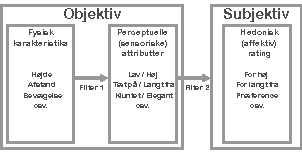
\includegraphics[width = 0.9\textwidth]{Figure/Filter} 
\caption{Filter model for det objektive: Fysiske karakteristika og attributter samt det subjektive: Hedonisk rating.}
\label{fig:Filter}
\end{figure}
\noindent
%
Filter modellen afbilledet på \autoref{fig:Filter} bygger på modellen fremsat af \textcite[s. 4]{PDF:AttributeIdentificatoin}. Denne model bygger på input og output for de to filtre, hvor inputtet i det første filter er de fysiske karakteristikas af stimuli, som eksempelvis er højde, afstand, bevægelse. Outputtet af \textit{Filter 1} illustreres i boksen for perceptuelle attributter på \autoref{fig:Filter}, som er de attributter, der er udledt fra testpersonernes respons. Dernæst er inputtet til \textit{Filter 2} de udviklede skalaer, som bygger på de fundne attributter, hvor outputtet af \textit{Filter 2} er den subjektive evaluering af interaktionen med robotten angivet på de udviklede skalaer. 


